\chapter{Генерация изображений с помощью методов машинного обучения}
\section{Диффузионные нейронные сети для генерации изображений}

Генерация изображений с помощью нейронных сетей сегодня играет важную роль в развитии
информационных технологий, позволяя автоматизировать создание иллюстраций.
Широкое распространение генеративных технологий стало возможно благодаря улучшению методов обучения нейронных
сетей, которые решают данную задачу, и развитию вычислительной техники.

Выделяют различные виды задач генерации изображений:
\begin{enumerate}
  \item Генерация изображений по заданному текстовому описанию (промпту), которую в англоязычной литературе называют inpainting.
  \item Генерация фона по промпту, которую в англоязычной литературе называют outpainting. Обе перечисленных
  задачи сокращенно называют text2image.
  \item Генерация изображений по заданному изображению и промпту, которая находит применение в фильтрах обработки фотографий с помощью нейронный сетей. 
\end{enumerate}

При использовании текстовых промптов в качестве входных данных в первую очередь решается задача представления текста в виде векторов
чисел. 
Для этого используются токенайзеры, возможно, в комбинации с небольшими языковыми моделями.
Данный этап также представляет ценность на этапе обучения и позволяет распознавать запросы на разных языках и системах
письменности без использования нормализации и перевода.

В данной работе в первую очередь рассматривалась задача inpainting на примере маленьких открытых моделей семейства
stable diffusion, поскольку они позволяют продемонстрировать основные проблемы, связанные с инференсом изображений
при высокой нагрузке, но не требуют больших вычислительных ресурсов и просты в эксплуатации.

Одним из значимых методов обучения нейронных сетей, предназначенных для генерации изображений, стал Generative adversarial network (GAN).
Ключевой особенностью данного метода на этапе обучения является наличие двух глубоких нейронных сетей: $G(z)$, которая по распределению $p_g$ ставит
в соответствие векторам $z$ изображения $x$, и сети $D(x)$, которая возвращает скалярное значение,
которое является вероятностью того, что $x$ является реальным изображением, то есть является частью
обучающей выборки. 
Основная идея процесса обучения заключается в минимизации величины $\log (1 - D(G(z)))$, что означает, что $G$ пытается «обмануть» дискриминатор $D$.
Поэтому подобный подход к обучению нейронный сетей можно считать обучением без учителя. 

Таким образом процесс получения распределения $p_g$ можно представить в виде игры с нулевой суммой двух игроков
с критерием \cite{gan}
$$
\min_{G}\max_{D} V(D, G) = \mathbf{E}_{x~p_{data}(x)}[\log D(x)] + \mathbf{E}_{z~p_{z}(z)}[\log (1 - D(G(z)))]
$$ 

Данный подход гарантирует сходимость при увеличении обучающей выборки и обеспечивает хорошую скорость инференса относительно подходов,
основанных на других вероятностных методах, но является очень трудозатратным при обучении модели.

Поэтому наряду с GAN часто применяются диффузионные модели (Dif\-fusion models), принцип которых основан на 
итеративном извлечении шума с изображения, что позволяет создавать из шума искомые изображения.
\section{Латентные диффузионные нейронные сети для генерации изображений}


Важную роль процессе уменьшения шума в изображении играет сегментация изображений с помощью U-Net нейронных сетей,
которые имеют большое значение в биоинформатике.

Основная идея U-Net заключается в последовательном использовании блоков конволюции и деконволюции вместе с ReLU 
функциями активации (Рисунок \ref{fig:unet}), при котором разрешение исходного изображения последовательно понижается, а потом повышается
до исходного. 


\begin{figure}[H]
  \centering
  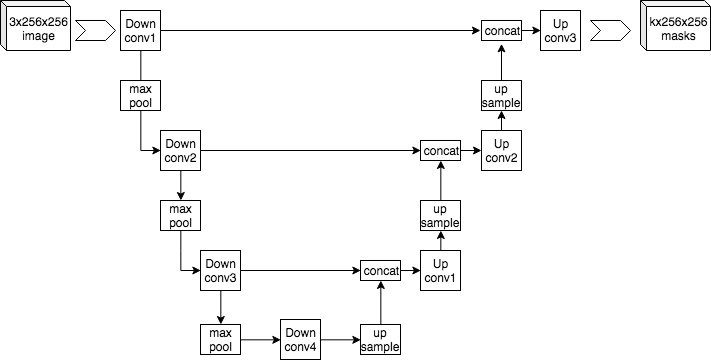
\includegraphics[width=0.95\textwidth]{img/unet.png}
  \caption{--- U-Net \cite{rombach2022high}}
    \label{fig:unet}
\end{figure}


В результате данных преобразований на изображении выделяются основные детали, соответствующие отдельным объектам (Рисунок \ref{fig:conv}), а полученное изображение,
как правило, называют маской. В контексте использования диффузионных моделей для генерации изображений использование
сегментации на зашумленных изображений помогает более эффективно избавляться от шума, что улучшает сходимость процесса генерации.

\begin{figure}[H]
  \centering
  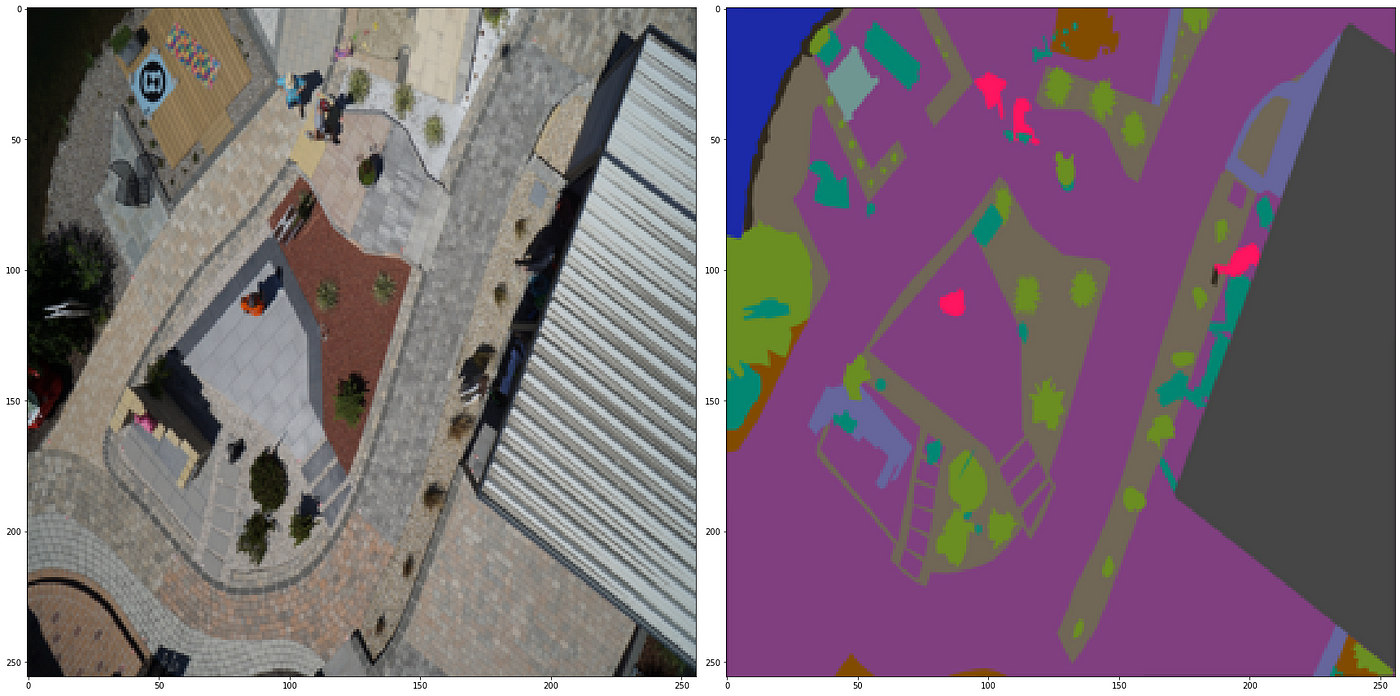
\includegraphics[width=0.95\textwidth]{img/conv.png}
  \caption{--- Результат применения U-Net на изображении}
    \label{fig:conv}
\end{figure}

Комбинацию подходов сегментации изображений между шагами генерации зачастую выделяют в отдельный тип нейронных сетей, называемый
латентными диффузионными моделями (Latent Diffusion Models). Латентными их называют за счет того, что латентным называют пространство
изображений, получаемых в ходе шагов семплирования, с применением конволюции и деконволюции U-Net. Это значительно
упрощает обучение модели и позволяет сразу генерировать изображения в высоком разрешении против подходов, где применяется
комбинация нескольких нейронных сетей, где на определенных шагах формируются детали, а на конечных повышается разрешение
до искомого (Рисунок \ref{fig:latent}).
LDM лежат в основе большинства современных нейронных сетей,
которые решают задачу генерации изображений, таких как DALLE, Midjourney и YandexART.
\begin{figure}[H]
  \centering
  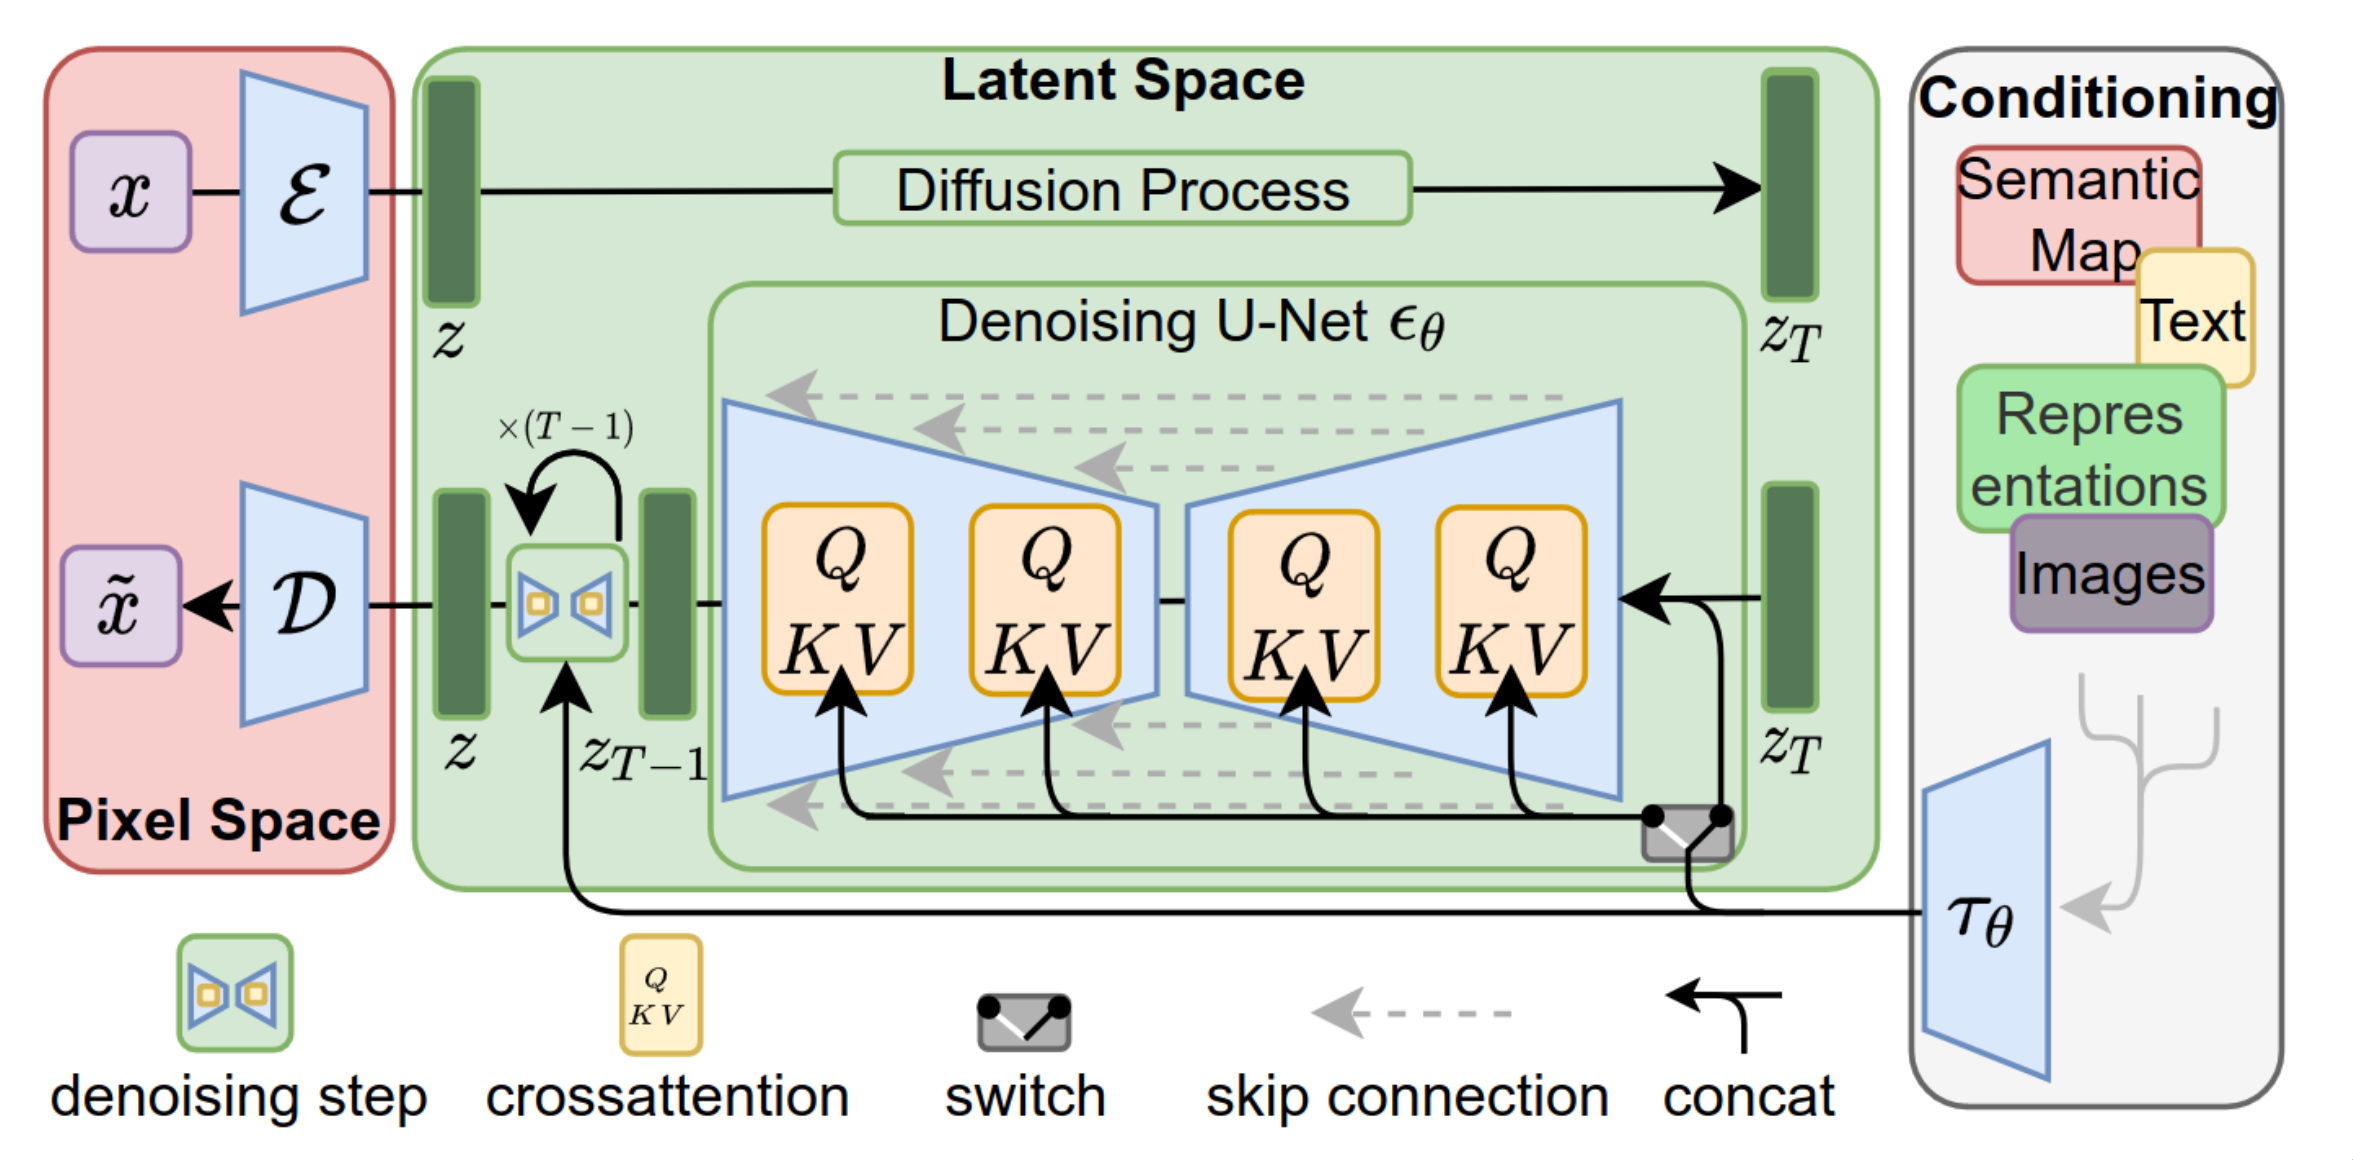
\includegraphics[width=0.95\textwidth]{img/latent.png}
  \caption{--- Схема архитектуры LDM\cite{rombach2022high}}
    \label{fig:latent}
\end{figure}

Несмотря на применение вышеперечисленных оптимизаций,
генерация высококачественных изображений доступна только на высокопроизводительных GPU промышленнного сегмента,
представленными, например, NVidia V100, A100, H100 и так далее. 
Данные вычислительные устройства производятся в ограниченном количестве и являются относительно дорогими,
что делает невозможным обработку множества запросов в режиме реального времени, что требует выстроения инфраструктуры
вокруг моделей, которая сможет обеспечить бесперебойную и асинхронную обработку сообщений, 
соответствующую по пропускной способности количеству вычислительных ресурсов.
Также при большом количестве RPS (requests per second) на генерацию встает вопрос о масштабирования кластера
видеокарт. 

Одним из возможных сценариев масштабирования вычислительных ресурсов является создание суперкомпьютеров с объединением
шины данных нескольких видеокарт. Подобные технологии представлены в потребительском сегменте технологиями SLI от компании NVidia и CrossFire от AMD, однако
данные технологии в первую очередь предназначены для неспециализированных вычислений, которые, например, нужны для
отрисовки графики в видеоиграх и не всегда подходят для сложных вычислительных задач, а так же не предоставляют достаточную скорость
обмена данными между видеокартами. Подобные подходы так же критикуются за счет того, что производительность таких систем не растет линейно и
требуют высоких накладных расходов на синхронизацию работы нескольких видеокарт.

Поэтому в качестве альтернативного способа создания кластеров видеокарт зачастую применяют технологию NVLink, которую разработала 
компания NVidia (Рисунок \ref{fig:nvlink}). Она не предназначена для решения задач общего назначения, поэтому видеокарты с поддержкой NVlink не всегда обладают 
мультимедийными интерфейсами, типа HDMI или DisplayPort, однако предоставляет в 3 раза большую частоту передачи данных
по сравнению с видеокартами с интерфейсом подключения PCIExpress 3.0 на примере видеокарт серии V100.

Данный подход может обеспечить максимальную производительность за счет минимизации передачи данных по сети
и предоставляет самый эффективный механизм вертикального масштабирования. Объединение видеокарт в кластеры на аппаратном
уровне может быть необходимостью при обучении больших моделей или инференсе моделей, которые не помещаются целиком
в память одной видеокарты, однако может быть излишним для инференса небольших, до 40-80 гигабайт, обученных моделей,
поскольку проектирование подобной системы на физическом уровне может быть очень затратным и имеет пределы, диктуемые
сетевой аппаратурой и контролерами, в которые подключается кластер видеокарт.

\begin{figure}[H]
  \centering
  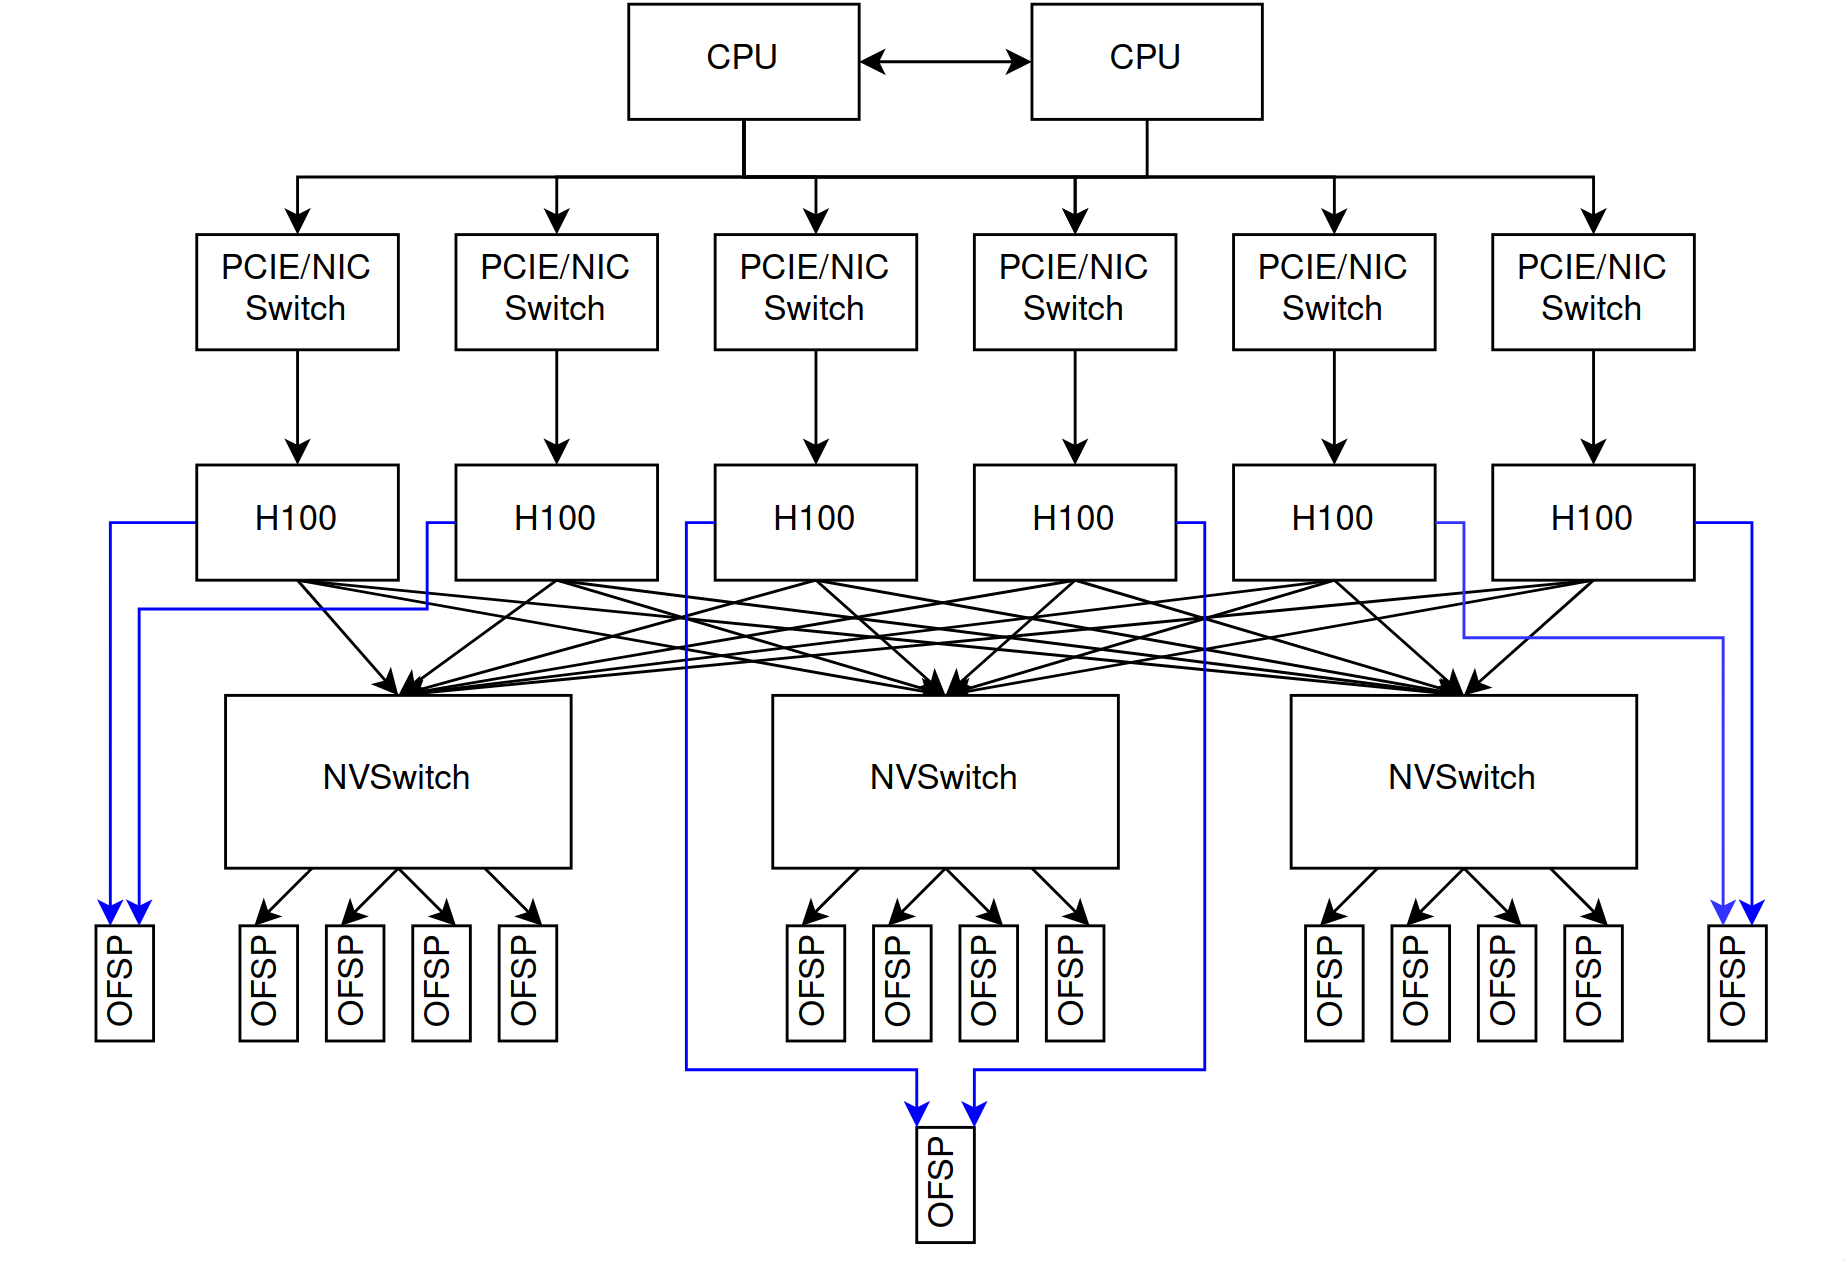
\includegraphics[width=0.95\textwidth]{img/nvlink.png}
  \caption{--- NVlink кластер}
    \label{fig:nvlink}
\end{figure}


В качестве альтернативы аппаратному кластеру видеокарт можно использовать архитектуру, в которой видеокарты не объединяются
в аппаратный кластер, а обладают независимыми шинами данных, а координация их работы обеспечивается на уровне приложения.
Данный подход позволяет разнести вычислительные ресурсы на разные машины и не требует более сложной инфраструктуры, связанной
с обслуживанием оборудования, соответственно, предоставляет более простые механизмы горизонтального масштабирования,
что может помочь в построении больших систем. Видеокарты, которые работают по отдельности, также не нуждаются в 
NVlink и могут быть подключены через более дешевый и простой в эксплуатации PCIExpress.
С другой стороны, такой подход может не подойти для сценариев, где модель не помещается в память одной видеокарты, и координация
работы составной нейронной сети будет медленнее, чем в системе с несколькими видеокартами, за счет необходимости
передачи данных по сети. Еще можно заметить, что видеокарты предназначенные для PCIExpress обладают более медленной
памятью, поэтому, на примере видеокарт H100, при одинаковых характеристиках чип будут показывать худшую производительность
при решении вычислительных задач.

В случае если к системе не предъявляется вышеперечисленных требований, предпочтительным является именно этот подход за счет своей простоты.
Самым простым в реализации будет построение архитектуры, где общение с моделями осуществляется через балансер, который
держит ограниченный пул соединений с HTTP-серверами моделей. Обеспечение HTTP API для модели обеспечивается пользователем
на уровне приложения или используется готовое решение, типа TorchServe, который обеспечивает батчинг запросов и конфигурацию без
без необходимости реализации этого программистом.

\begin{figure}[H]
  \centering
  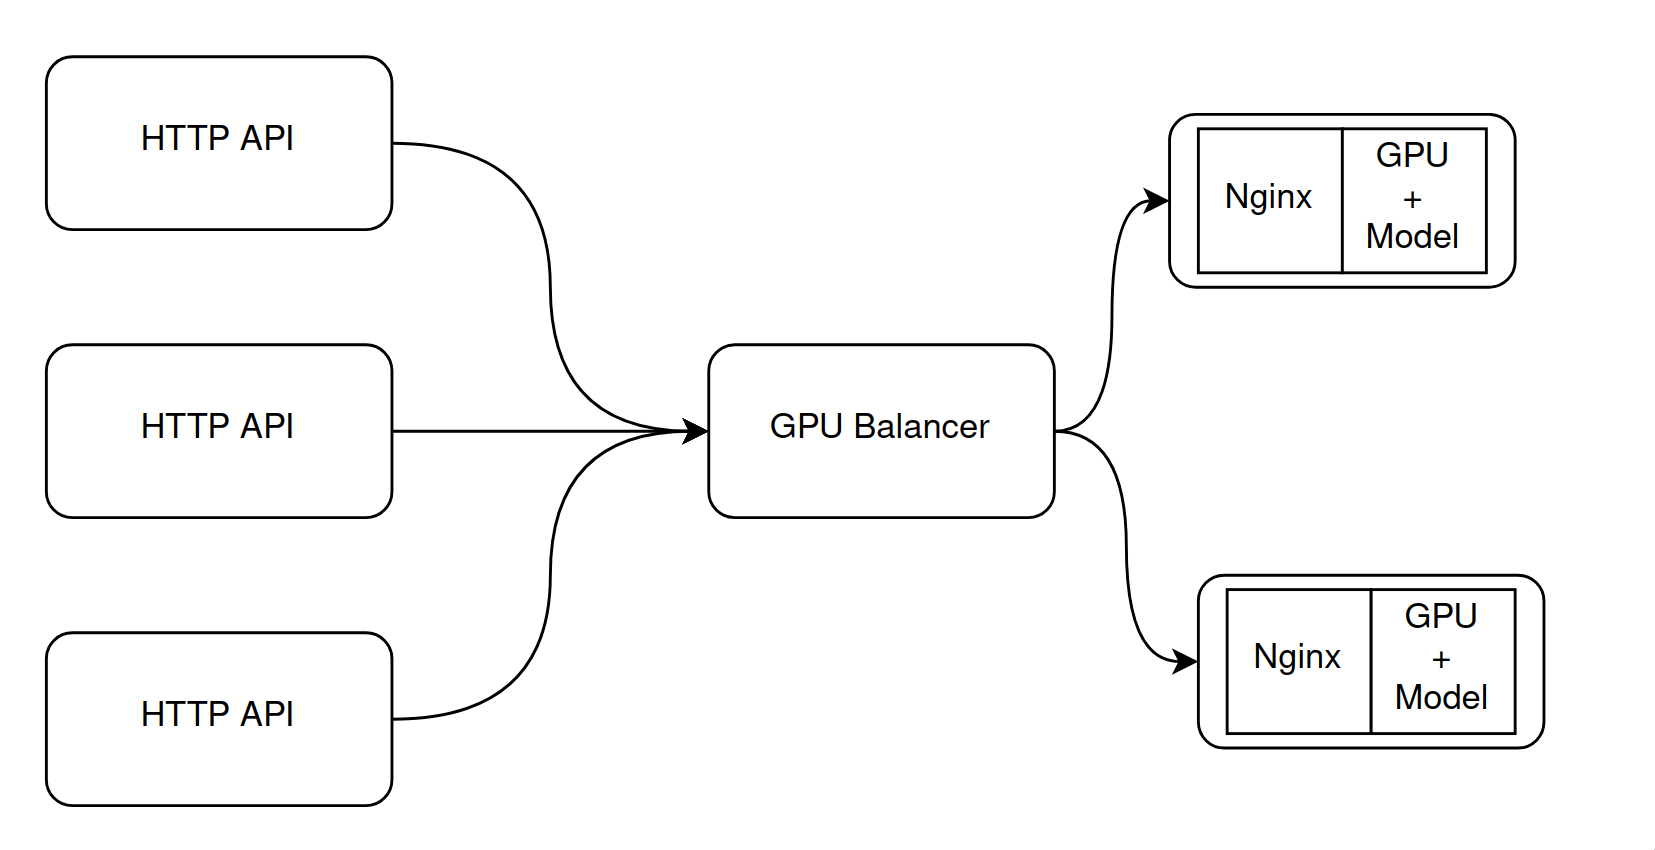
\includegraphics[width=0.95\textwidth]{img/gpu_balancer.png}
  \caption{--- Балансер}
    \label{fig:balancer}
\end{figure}

Использование общего балансера может упростить инфраструктуру системы и код для эксплуатации модели, однако налагает
серьезные ограничения на отказоустойчивость системы: при большом количестве RPS на генерацию может не хватать 
соединений, за счет того, что на каждый запрос, который не может быть обработан сразу из-за отсутствия свободных ресурсов,
будет выделено отдельное соединение, тратящее процессорное время. Также релизный цикл обновлений модели
будет требовать сложной конфигурации систем деплоя, типа Kubernetes, для обеспечения бесперебойной обработки запросов (Green-Blue Deployment).
Иначе текущие запросы будут обрываться в процессе обновлений.

В качестве альтернативы можно дополнить данную схему отдельной очередью, что позволит обрабатывать сообщения асинхронно, а 
гарантии обработки обеспечивать за счет механизмом подтверждения на уровне брокера сообщений, который выступает в роли очереди.

В данном случае HTTP-прокси будет заменен на интерфейс взаимодействия с брокером сообщений, написанный на языке 
рантайма инференса, или на другом языке программирования. В последнем случае обработка сообщений и инференс модели
будут происходить в разных процессах на одной физической модели, а приложения для взаимодействия с брокером сообщений называется 
Sidecar.

\begin{figure}[H]
  \centering
  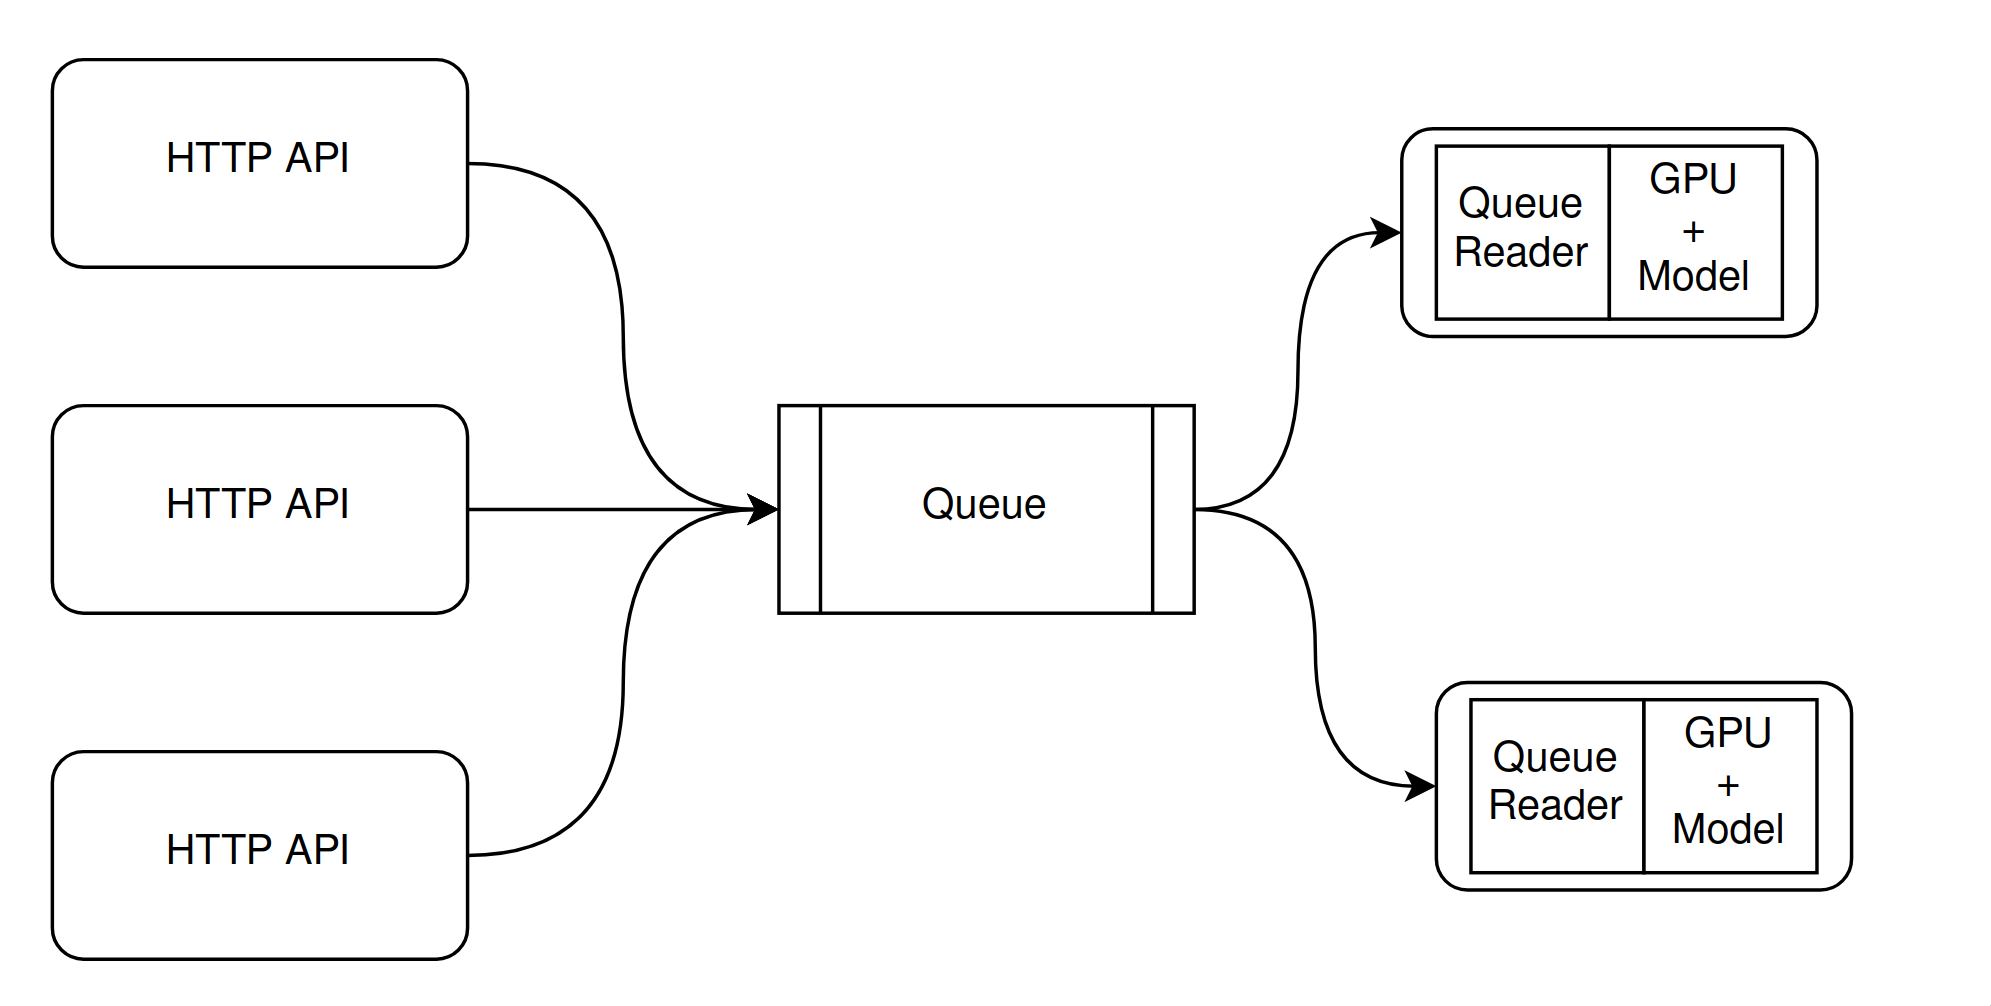
\includegraphics[width=0.95\textwidth]{img/queue.png}
  \caption{--- Очередь}
    \label{fig:queue}
\end{figure}

В качестве преимуществ данного подхода можно выделить более простую обработку сценариев с высокой нагрузкой
и обработкой ошибок на стороне модели за счет подтверждений на стороне брокера сообщений и его персистентного хранилища,
которое будет хранить информацию о запросе установленное время даже после перезапуска приложения. Использование
очереди также может обеспечить гарантии очередности обработки сообщений, что дает более предсказуемое время ожидания
под высокой нагрузкой. 
